\documentclass[a4paper, 12pt, oneside]{book}
\usepackage[margin=1in]{geometry}
\usepackage{amsmath}
\usepackage{enumitem}
\usepackage{float}
\usepackage{graphicx}
\usepackage{tabularx}
\usepackage{setspace}
\usepackage{amsmath}
\usepackage{fancyvrb}
\newcommand*\diff{\mathop{}\!\mathrm{d}}
\usepackage{titlesec}
\usepackage{hyperref}
\usepackage{listings}
% \setlist{itemsep=0pt,parsep=0pt}
\setlength{\parindent}{0pt}

% set alphabet enumeration
\setcounter{secnumdepth}{3}
\setcounter{tocdepth}{2}
\renewcommand\thesubsubsection{\alph{subsubsection}} 
\makeatletter
\renewcommand\p@subsubsection{\thesubsection.} 
\makeatother

\hypersetup{
    colorlinks,
    citecolor=black,
    filecolor=black,
    linkcolor=black,
    urlcolor=black
}


% title setup
\title{Part IB Summer Work}
\author{Athena Eng}
\date{}


% begin document
\begin{document}

\maketitle
\tableofcontents

\newpage

(If I happen to do more/decide to explain myself for this work I'm submitting: \url{https://github.com/Athena-E/Athena_IB_summer_work_answers})

\newpage

\chapter{Computer Architecture}

\section{Threshold Warning System Design}
We need to trigger a warning if the weighted sum of a time-varying input signal exceeds some
threshold.

\subsubsection{Analogue System}\label{a}

The value to compare with the threshold is given by the integral over time:

\[V_{\text{out}}(\tau)=\int_{0}^{\tau}w^{\tau-t} \cdot V_{\text{in}}(t) \diff t,\]

where $w < 1$ and $\tau$ is the current time.\\

We can approximate the integral as the Riemann sum using the recurrence relation:

\[V(\tau) = V_{\text{in}}(\tau) + {w^T}\cdot V(\tau-1)\]

and multiplying by the time period:

\[V_{\text{out}}(\tau) = T \cdot V(\tau), \]

where $T$ is the time period of the input voltage.\\

Using an adder circuit and choosing suitable resistor values, we can compute the weighted sum, as per the recursive equation.

\[V_t = -\left(\frac{V_{in}}{R_1} + \frac{V_{t-1}}{R_2}\right)\cdot R_3\]

Let $R_1 = R_3 = 1$, $R_2 = w^T$,

\[V_t = -\left({V_{in}} + w^T\cdot {V_{t-1}}\right)\]

\begin{figure}[H]
  \centering
  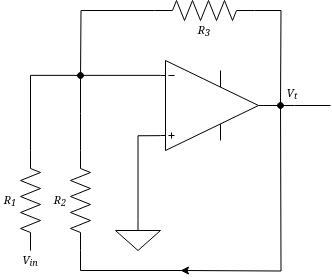
\includegraphics[scale=0.5]{adder.png}
  \caption{Adder circuit}
\end{figure}

We then multiply the result of $V_t$ with the time period of the input voltage before comparing with the threshold. This can be done by using log, antilog and summing amplifiers.\\

For the log amplifier, the relationship between the input voltage, $V_i$ and output voltage, $V_0$ is expressed as:

\[V_0 = -V_T \ln \left(\frac{V_i}{I_S R}\right),\]

\begin{figure}[H]
  \centering
  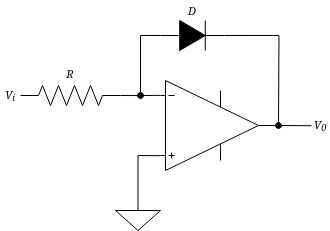
\includegraphics[scale=0.5]{log.png}
  \caption{Log amplifier}
\end{figure}

where $I_S$ is the saturation current and $V_T$ the thermal voltage of the diode.

For the antilog amplifier, the relationship between the input voltage, $V_i$ and output voltage, $V_0$ is expressed as:

\[V_0 = -R I_S \cdot e^{(V_i/V_T)}\]

\begin{figure}[H]
  \centering
  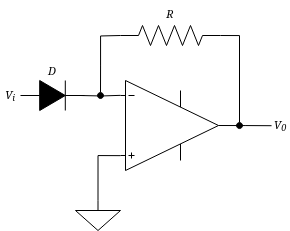
\includegraphics[scale=0.5]{antilog.png}
  \caption{Antilog amplifier}
\end{figure}

We will use an inverting summing amplifier to add the log of the output of the adder circuit and the log the time period.

\begin{figure}[H]
  \centering
  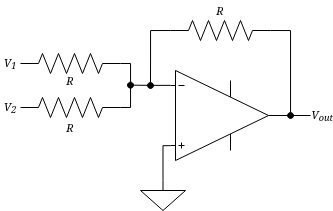
\includegraphics[scale=0.5]{summing.png}
  \caption{Inverting summing amplifier}
\end{figure}

An inverter will be used before the final comparator to ensure that $V_{\text{out}}$ is positive.

\begin{figure}[H]
  \centering
  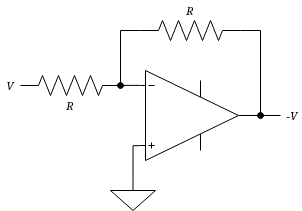
\includegraphics[scale=0.5]{inverter.png}
  \caption{Inverting amplifier}
\end{figure}

\begin{figure}[H]
  \centering
  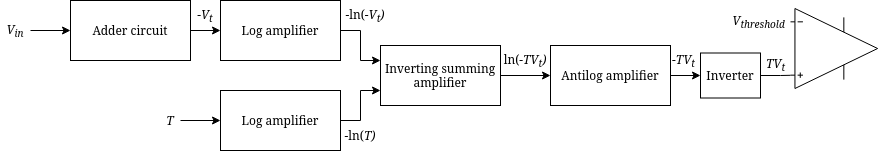
\includegraphics[scale=0.5]{full_circuit.png}
  \caption{Full circuit}
\end{figure}

% \begin{center}
%   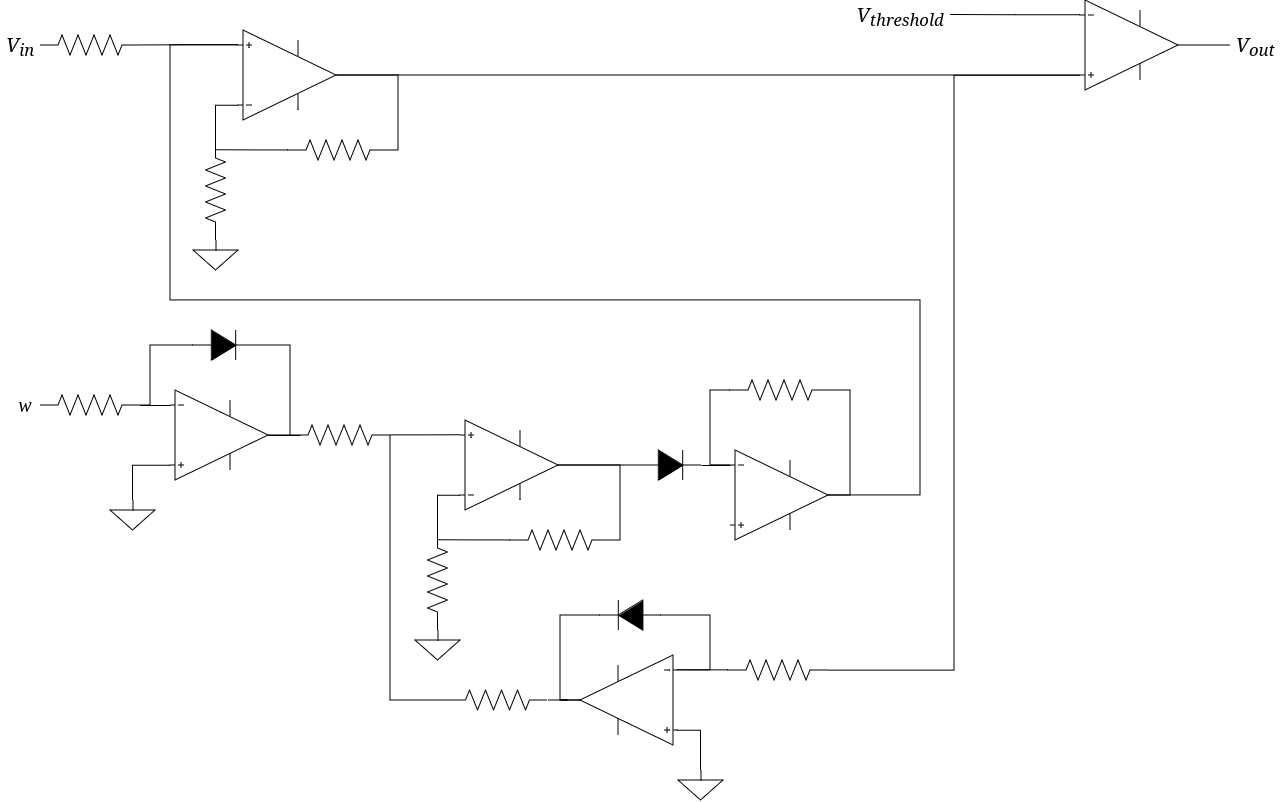
\includegraphics[scale=0.3]{analogue.png}
% \end{center}

% The circuit uses operational amplifiers and combines logarithmic, exponential and summing amplifiers to compute the weighted sum, as per the recursive equation above.

\subsubsection{Digital System}\label{b}

The input is a 32-bit floating point value that can be read into CPU register 0. The weight is stored in \texttt{r1} and the threshold in \texttt{r2}. The program stores -1 to address \texttt{0x1337d00d} whenever the weighted sum exceeds the threshold (and 0 when not breached). The same recursive equation used for the analogue system can be used for the digital solution, expressed as a a machine code loop.\\
\\
\textbf{Instruction set:}
\begin{table}[H]
  \centering
  \begin{tabularx}{\textwidth}{|X|X|}
    \hline
    \texttt{LDR rd, <memory ref>}   & Load the value stored in the memory location specified by \texttt{<memory ref>} into register \texttt{d}.                            \\
    \hline
    \texttt{STR rd, <memory ref>}   & Store the value that is in register \texttt{d} into the memory location specified by \texttt{<memory ref>}.                          \\
    \hline
    \texttt{ADD rd, rn, <operand2>} & Add the value specified in \texttt{<operand2>} to the value in register \texttt{n} and store the result in register \texttt{d}.      \\
    \hline
    \texttt{MUL rd, rn <operand2>}  & Multiply the value specified in \texttt{<operand2>} to the value in register \texttt{n} and store the result in register \texttt{d}. \\
    \hline
    \texttt{CMP rn, <operand2>}     & Compare the value stored in register \texttt{n} with the value specified by \texttt{<operand2>}.                                     \\
    \hline
    \texttt{B<condition> label}     & Branch to the instruction at position \texttt{label} if the condition is met at the last comparison.                                 \\
                                    & \texttt{GT}: greater than                                                                                                            \\
    \hline
    \texttt{MOV rd, <operand2>}     & Copy the value specified by \texttt{<operand2>} into register \texttt{d}.                                                            \\
    \hline
    \texttt{\#}                     & Immediate addressing mode                                                                                                            \\
    \hline
  \end{tabularx}
\end{table}

\begin{verbatim}
loop:
  LDR r0, [0xdeadbeef]
  MUL r4, r3, r1    ;multiply weight with accumulated sum, store in r4
  ADD r5, r0, r4    ;add weighted sum to input, store in r5
  CMP r5, r2        ;compare with threshold
  BGT exit
  MOV r4, r5        ;update weighted sum in r4
  B loop
exit:
  STR #-1, [0x1337d00d]
\end{verbatim}

The machine code uses a loop to calculate the weighted sum as new inputs are loaded into \texttt{r0}. The weighted sum of the inputs, bar the most recent, is stored in \texttt{r4}. This is used to calculate the updated weighted sum with the new input and compared with the threshold in \texttt{r2}. When the weighted sum is greater than the threshold, the loop exits and \texttt{-1} is stored to \texttt{[0x1337d00d]}.


\section{Calculating the factorial of an integer input}

\subsubsection{Accumulator Architecture}

Accumulator machines store the majority of results from calculations in the designated accumulator register. They are `1-operand machines', as the accumulator register is usually an implicit operand.\\

Arithmetic instructions are performed on a given memory address and the accumulator, which replaces the contents of the accumulator with the result. To calculate the factorial of an integer $n$ with an accumulator architecture, we need a register to store a running value of the factorial and a register to store the current value of $n$ in the iterative calculation. The input is assumed to be a non-negative integer.

\begin{Verbatim}[numbers=left,xleftmargin=5mm]
  BR 3            ;check if input is 0
  LDIMM 1         ;set accumulator to 1 if input 0
  STORE [0x10]    ;running value
  STORE [0x11]    ;current n
  LDIMM 1
  MUL [0x10]
  STORE [0x10]    ;update running value
  LDIMM -1
  ADD [0x11]      ;calculate n-1
  STORE [0x11]    ;update n to n-1
  BR 6
  LOAD [0x10]     ;load final result to accumulator
  END
\end{Verbatim}

Lines 4-9 represent the loop, which calculates $n\times(n-1)\times...\times1$ until the current value of $n$ stored at \texttt{0x11} is 0, at which point the loop terminates and the integer stored at \texttt{0x10} is the final result. To handle the edge case $0! = 1$, the accumulator is set to 1 if the input is 0, as controlled by the branch instruction on line 1.

\subsubsection{Stack Architecture}
A stack machine uses a push down stack to store operands and results. Most of the opcodes in a stack machine instruction set do not have explicit operands, as operations are performed on operands in the stack based on the order in which they were pushed. This is zero address formatting and can help reduce the number of registers required for hardware processing.\\

The instruction set for a stack machine carries out arithmetic instructions with postfix operations since postfix expressions can be evaluated using a stack. Hence, it would be convenient to construct a stack containing \texttt{[n, n-1,...,1]} before repeatedly applying the multiplication operator until only the final result is left on the stack. The only branching instruction \texttt{BR} $m$, which provides us with some form of selection, removes the top of the stack and if it is non-zero, the next instruction is at line $m$. It is easy to construct a stack (starting from the top) \texttt{[0,1,2,...,n]} and the branch operation can indicate when construction can terminate. To indicate when the muliplication of elements can terminate, we will actually construct the stack \texttt{[0,1,2,...,n,0]} so that when we can terminate once we have reached the bottom of the stack.

\begin{Verbatim}[numbers=left,xleftmargin=5mm]
  DUP
  BR 5        ;handle input 0
  POP
  PUSHIMM 1   ;input 0 same as input 1
  PUSHIMM 0
  SWAP        ;put 0 at bottom of stack
  DUP         ;start of loop to construct stack
  PUSHIMM -1
  ADD
  DUP
  BR 7        ;end of loop
  POP         ;remove 0
  MUL         ;start of loop to multiply
  SWAP
  DUP
  BR 13       ;end of loop
  POP         ;remove 0
  END
\end{Verbatim}

\subsubsection{Register Architecture}

\begin{Verbatim}[numbers=left,xleftmargin=5mm]
  BR r0, 2          ;handle input 0
  LDIMM r0, 1
  LDIMM r1, 0
  LDIMM r2, -1
  ADD r1, r0, r1    ;copy value of n to r1
  LDIMM r0, 1
  MUL r0, r0, r1    ;start of loop to multiply
  ADD r1, r1, r2    ;calculate n-1
  BGT r1, -2        ;end of loop
  END
\end{Verbatim}

This is similar to the solution for the accumular architecture, where most results are stored in \texttt{r0} and the decrementing next value starting from the initial input is stored in \texttt{r1}.

\section{Pipeline Performance Analysis}
For an instruction pipeline that can be divided perfectly into $s$ balanced stages, the cycle time $\tau$ is defined as:

\begin{align*}
  \tau & = \max_{1\le i\le s}\tau_i + d \\
       & = \tau_m + d,\
\end{align*}

where $\tau_m$ denotes the maximum stage delay (which should be the same for every stage in this situation) and $d$ denotes the latching delay when advancing signals from one stage to the next. If $T$ is the total execution time for a single instruction in a non-pipelines processer, then $\tau_m$ is given by:

\[\tau_m = \frac{T}{s}\]

Hence, the number of instructions issued per second $I$ is equal to:

\[I = \frac{1}{\frac{T}{s} + d}\]

\subsubsection{Intel Pentium Mobile vs. Intel Xeon}
Having more pipeline stages means that each individual stage can be implemented with simpler circuitry, which may let the processor clock run faster.\\

The Intel Pentium Mobile family of processors is largely designed for general-purpose use, whereas the Intel Xeon family of processors is used in high-performance computing environments and mission-critical applications.\\

The Intel Xeon processor is likely to have more pipeline stages, since it is often used in real-time systems. The increased clock speed allows more instructions to be completed per unit time. Applications such as servers and data centers receive require large throughput to handle incoming requests, which would make the most of increased pipeline stages.

\subsubsection{Branch Instructions and ALU Operations Ratio}
Given a 7-stage pipeline and a 21-stage pipeline:\\

7-stage microarchitecture: IF, DE, EX1, EX2, EX3, MA1, WB\\
21-stage microarchitecture: IF, DE1, DE2, DE3, EX1, EX2, .. EX14, MA1, MA2, WB\\

We assume that each stage in the 7-stage pipeline has a cycle time of 3 units and the 21-stage pipeline has a cycle time of 1 unit, such that both pipelines have the same total time to complete an ALU operation. Without any branch instructions, the 21-stage pipeline outperforms the 7-stage pipeline since its throughput (after the first operation) is every 1 unit of time whereas the 7-stage pipeline has a throughput of every 3 units of time. With branch instructions, the pipeline stalls until the final EX stage is reached in either pipeline.\\

We will use CPI to compare the pipelines. The ideal CPI in a pipeline is 1, but with stalls the CPI will be expressed:

\begin{align*}
  \text{CPI pipelined} & = \text{Ideal CPI} + \text{Pipelines stall clock cycles per instruction} \\
                       & = 1 + \text{Pipelines stall clock cycles per instruction}
\end{align*}

For the 7-stage pipeline, which stalls for 4 cycles for every branch instruction:

\begin{align*}
  \text{CPI pipelined} & = 1 + 4 \times \frac{b}{a+b}
\end{align*}

where $b$ denotes number of branch instructions, $a$ the number of ALU instructions.

Similarly for the 21-stage pipeline, which stalls for 17 cycles:

\begin{align*}
  \text{CPI pipelined} & = 1 + 17 \times \frac{b}{a+b}
\end{align*}

We now compare the cycle time per instruction and determine the ratio by solving the inequality:

\begin{align*}
  3 \times  \left(1 + 4 \times \frac{b}{a+b}\right) & < 1 + 17 \times \frac{b}{a+b} \\
  2a                                                & < 3b
\end{align*}

which suggests a ratio of ALU to branch instructions greater than $3:2$ for the 7-stage pipeline to outperform the 21-stage pipeline.

\section{Pipeline Data Hazards}

\subsubsection{No Feed-forward Paths}

\textbf{Read After Write (RAW) Hazard}\\

RAW Hazards occur when an instruction depends on the result of a previous instruction that has not yet been written back.\\

A LOAD instruction followed by an ALU operation may result in a hazard if the ALU operation requires a register value that has not yet been loaded by the ALU operation's execution stage:
\begin{verbatim}
  LOAD r1, #0xdeadbeef       ;load r1 during WB stage
  ADD r3, r1, r2             ;requires r1 in DE stage
\end{verbatim}

Similarly, an ALU operation followed by another ALU operation can result in a hazard if both operations have the same register as an operand:
\begin{verbatim}
  ADD r0, r1, r2    ;write r0 during WB stage
  ADD r3, r0, r4    ;requires r0 in DE stage
\end{verbatim}

\textbf{Write After Write (WAW) Hazard}\\

WAW Hazards occur when multiple instructions write to the same register and the order of writing has an effect.

Successive ALU operations that write to the same register will cause this hazard:
\begin{verbatim}
  ADD r0, r1, r2    
  ADD r0, r3, r4    ;must delay WB until execution of first instruction
\end{verbatim}

An ALU operation that shifts its second operand and an ALU operation that writes to this same operand will cause this hazard, as the shift stage overwrites a register value:
\begin{verbatim}
  ADD r0, r1, r2
  ADD r3, r4, r0<<r5    ;must delay shift until r0 written to
\end{verbatim}

The ADD operation writes to the r0 register during its shift operand 2 stage before the LOAD operation has time to reach the write back stage and write to r0 first.
\begin{verbatim}
  LOAD r0, #0xdeadbeef
  ADD r1, r2, r0<<r3
\end{verbatim}

\textbf{Write After Read (WAR) Hazard}\\

WAR Hazards occur when an instruction writes to a register that a previous instruction reads from but before the read completes.

An ALU operation that reads from a register whos value is shifted in a following instruction may cause this hazard if the value is shifted by the latest ADD operation if the previous ADD operation has finished reading from it (execute and shift operand stages interfere).
\begin{verbatim}
  ADD r5, r6, r1
  ADD r2, r3, r1<<r4
\end{verbatim}


\subsubsection{Feed-forward Path}

Feed-forwarding allows pipelines to bypass the normal flow of data and pass results directly from one pipelined instruction to another when it becomes available. For instructions that require the result of an ALU result, feed-forwarding eliminates need for stalls and bubbles. Bubbles will still be required when instructions are waiting to read from registers that LOAD (and potentially STORE instructions) have not written to yet.\\

By the execute stage, the ADD operation needs to read r0, which will not be available until the write back stage of LOAD. At the ADD operation's execute stage, the LOAD operation will only be at its memory access stage
\begin{verbatim}
  LOAD r0, #0xdeadbeef
  ADD r1, r2, r0
\end{verbatim}

\section{Pipeline Instruction Decode Stage Algorithm}

An algorithm that determines whether the next instruction coming out of the instruction decode stage can continue without a pipeline bubble would need to maintain state of the registers required by this next instruction; link between registers and prior instructions which may be reading from/writing to them; the stage of these instructions; and whether there are any values that are being fed forward to the next instruction. Given that the next stage is the shift operand 2 stage, we focus on the state of the second operand. The decode stage will determine whether the second operand needs to be shifted in the following stage; if it does not, the instruction will be allowed to issue since the availability of operand 2 is not relevant.\\
\\
For STORE and LOAD instructions that write to a register that is required by the next instruction, the register will only be available after the final write back stage. For ALU operations, the register at which the result is written to will be available after the execute stage. Thus, the algorithm must maintain state for an instruction's stage in the pipeline. Whether to proceed also depends on the optional shift operand if it is present, though unlike the register being shifted that is being written to, the shift operand register is only read from. We assume here that LOAD instructions only load from memory into registers and STR instructions only load from registers into memory. Hence, for STR instructions that read from a register that is also read by a next instruction as a shift operand, this condition still allows the instruction to be issued.

\begin{verbatim}
  REGS    # stores register indexes from instruction operands
  INST_TYPE   # stores instruction type [STR, LD, ALU]

  # stores registers with instruction that is currently using it
  REG_INST_TABLE

  op_2 = REGS[-2]   # get operand 2
  shift_op = REGS[-1]   # get shift operand if exists (else None)

  function check_shift_op():
    if REG_INST_TABLE[shift_op] is None:
      return True
    elif check_for_feed_fwd(shift_op):
      return True
    else:
      active_inst = REG_INST_TABLE[shift_op]
      # check if shift operand is being written to
      if active_inst.dest == shift_op:
        if active_inst.type == ALU && active_inst.stage > 3:
          return True
        else:
          return False
      else:
        return True

  if !op_2.is_shift:
    return check_shift_op()   # operand 2 is not shifted 
  elif REG_INST_TABLE[op_2] is None:
    # register is not in use by any other instruction
    return check_shift_op()     
  elif check_for_feed_fwd(op_2):
    # value for the register has been fed forward 
    return check_shift_op()   
  else:
    active_inst = REG_INST_TABLE[op_2]
    # 0-indexed stages
    if active_inst.type == ALU && active_inst.stage > 3: 
      return check_shift_op()
    else:
      # return False for all other cases
      # where instruction must wait for final write back
      return False
\end{verbatim}

Deciding whether to proceed to the execute stage would likely be implemented in the shift operand stage to decrease the amount of computation carried out in the decode stage.\\

\textbf{Hardware Implementation}\\
TODO

\section{Branch Delay Slot \& Taken Branch Penalty}

A branch delay slot is an instruction slot following a branch instruction and is often occupied by an instruction that can execute independent of the preceeding branch operation. For example in the following pseudocode:

\begin{verbatim}
  loop:
    READ value from register
    READ value from register
    ADD values from both registers
  BRANCH to loop if result < 1000
  WRITE result to memory
  READ value from register
\end{verbatim}

a READ instruction is read regardless of whether the branch is taken or not. This means it would be a suitable instruction to fill the instruction slot directly following the branch instruction. By the time the READ instruction has reached its decode stage, the result of the comparison will be ready and no time will have been wasted (i.e. no need for a bubble/NOP). The compiler/assembler will often include optimisations that rearrange the order of instructions (i.e. swap the order of the WRITE and READ instructions after the BRANCH). It can be challenging to choose a suitable instruction to fill the slot that is not dependent on the branch since there is limited time to search.\\

Taken branch penalty is the delay measured by the number of stages wasted in a branch misprediction. For example, in a 5-stage pipeline a branch misprediction results in a 2-stage branch penalty since the result of the branch is not known until its execute stage and instructions have the potential to be executed in parallel during its decode and execute stages. The branch misprediction results in killing the incorrectly fetched instruction and restarting the fetch at the actual target.\\

To reduce the number of branches executed (the dynamic count) to run a program, a compiler may implement optimisations that can rearrange the order of the low-level/intermediate representation to fill out branch delay slots and minimise branch penalties. There are many methods of compiler optimisations for branch prediction; for example, random branch prediction randomly reorders instructions involving branches such that a 50\% correct predication rate is guaranteed.



\section{CPU Cache Hierarchy}

\subsubsection{Cacheline Size}
Larger cache lines (128 bytes and above) are able to bring in more data with each cache miss and utilise spatial locality, which states that data with addresses that are near one another tend to be accessed close together in time. However, larger cache lines can result in wasted bandwidth if the data being brought in is not of the same fixed size as the cache line. \\

In multi-level caches, different cache line sizes can be used for each level; for example, level-3 cache may have a larger cache line than level-1 cache since it has a greater amount of storage and is able to exploit spatial locality more.

\subsubsection{Addressing: Virtual or Physical Addressing}
Using physical addressing for the tag and index of a cache entry avoids aliasing issues/synonyms where different virtual address may be mapped to the same physical addresses, and vice versa (homonyms*).\\

When using virtual addressing for the tag and index, synonyms can result in duplicated cache entries since different virtual addresses used to tag/index entries could map to the same physical address. Modifying any one of these entries may cause the other entries to become stale data, causing data inconsistency in the cache. However, virtual addresses have the benefit that they can be accessed immediately, in parallel with the TLB whereas physical addresses have to be translated to before they can be accessed; this means that virtual addressing has a faster access time. There is the issue that mappings between virtual and physical addresses may change, which would invalidate the tags/indices of cache entries.\\

Using virtually indexed, physically tagged caches overcomes the issue of homonyms since the physical tag can be used to discern physical addresses that may be mapped from the same virtual address. This method results in lower latency than PIPT since the cache line index can be looked up in parallel with TLB translation, though the tag cannot be used for comparison until the physical address has been looked up. This format may require more storage since the virtual and physical address will not necessarily have the same index bits. However, most VIPT caches are built not to have this issue and avoid incoherence by limiting the total number of bits for the index (and the block offset). As a result, the VIPT will have a size limited by the page size multiplied by the associativity of the cache.\\

The cost of dealing with virtual aliasing grows with cache size, so most level-2 and larger caches are physically indexed. Most level-1 caches are virtually indexed, which allows the MMU's TLB lookup to run in parallel for looking up a physically addressed tag, resulting in decreased latency.\\

% why does MMU not have to be consulted when going from virtual -> physical address?
% how does limiting no. bits for index help ensure virtual and physical addresses have same index (hence no need for extra storage)?
% why is size limited by pages size * associativity?
% why is PIVA useless? - is it because of VA synonyms and different indexes between physical and virtual addresses?

*Most modern processes manage homonyms by having a global address space for page table entries so that one virtual address does not map to multiple physical addresses. However, presence of homonyms means that different physical addresses cannot be indentified by consulting the cache index alone.

\subsubsection{Indexing: Direct-mapped, N-way Set-associative, Fully-associative}
Direct mapped caches map one block to one cache set; this makes block access very easy but puts constraints on the placement policy for where blocks can be placed since each memory address is mapped to just one cache set.\\

$N$-way set-associative caches map $N$ blocks to one set, where the tag is used to index the block within the set; the placement policy is able to choose between $N$ places in the cache.\\

Fully-associative caches have one set that all blocks reside in (so do not have any index bits, only tag bits); this means the placement policy can freely choose where to place blocks since all memory addresses are mapped to all cache sets.\\

(comment on implications for multi-level caches)

\subsubsection{Inclusivity: Inclusive, Exclusive, Non-inclusive-non-exclusive}

Inclusive cache design means that for multi-level caches, everything in L1 cache is also present in L2 cache (as an example). An advantage of inclusive cache is that when a process wishes to remove a line from cache, it need only check L2, as opposed to exclusive cache, which has to check both L1 and L2. However, if L2 does not have as many associative ways as all L1 caches, it can decrease the effective associativity of the L1 caches*. Additionally, if the L2 cache is evicted, those lines may also be present in the L1 cache, though not necessarily; finding these lines requires more work and will decrease the hit rate of the L1 cache. Although it may seem that more storage is required for inclusive cache, The larger L2 cache can have larger cache lines and the L1 cache does not need to have the same size cache lines as L2, unlike exclusive cache as this is needed to swap lines between the cache levels. The space saved on tag bits in the L1 cache line can make up for the space required to store data from L1 in L2 as well.\\

Exclusive cache design means that for multi-level caches, L1 and L2 do not share any data in common. The advantage of exclusive cache is that there is more available storage and is more beneficial when the size of L1 cache is comparable with L2 cache. When there is a cache miss, swapping a line in L1 with a line in L2 is more intensive than the copying process in inclusive caches.\\

Non-inclusive-non-exclusive cache means that data from L1 does not necessarily have to be present in L2 but it may often be so.

\subsubsection{Unification: Unified Cache, Instruction \& Data Caches (Split cache), Separate TLB}

Unified cache contains both instructions and data in the same cache; implementing actions to retrieve both instructions and data simultaneously requires multiple ports and more access time. In multi-level caches, an L2 cache could be a unified cache that receives forwarded service requests from a split L1 data cache and the L1 instruction cache. L1 cache is commonly split, given that the instruction cache can be placed nearer to the instruction fetch unit and the data cache can be placed near the memory unit, resulting in faster access times for both. However, it has been shown that split caches can result in higher hit rates since the combined space of both instruction and data caches may not be fully utilised. L2 and L3 caches often follow the unified design since they do not need to prioritise the same bandwidth and read capacity as they are not directly connected to the pipeline.

\subsubsection{Sharing: Shared, Private Caches}

Shared cache shares cache memory between cores of a multi-core processor as well as among different execution cores. In comparison with private caches which are each dedicated to a single core, the miss rate of shared cache decreases when cores do not require the same amount of cache. Private caches cannot share cache capacity under any circumstances, even if one core's cache has unused space that another core could make use of once its cache is full. When using a shared cache, a core can make full use of the L2 or L3 cache whilst the other cores are inactive. However, private caches have the advantage that they do not need a shared interconnect so there is lower latency for each core to access the cache as well as performance isolation.

\subsubsection{Write Policy: Write-back, Write-through}

The write policy determines the timing of when the cache performs a write to lower-level memory.\\

Write-through cache writes to lower-level memory after writing to cache every time. Write-back cache, writes are not immediate and instead marks overwritten entries as dirty. The data from these entries is then written to main memory once the cache has been evicted. Therefore, in a read miss, the cache may require two writes to memory; one to write the dirty location to memory and another to read the new location from memory.\\

(comment on implications for multi-level caches)

\subsubsection{Write misses: Write-allocate, Write-around}

A write-allocate policy allocates a cache line for a read or write miss in the cache. When data that is not in the cache needs to be written to a main memory location, a cache block is first allocated to that location before the data is written to cache. This avoids writing directly to main memory, which is slower than in the cache. In this policy, write misses act like read misses.\\

A write-around policy does not affect the cache, and the block is only modified in the lower-level memory. Blocks stay out of the cache until the program attempts to read the block, in which case space is allocated only when that event occurs.\\

Either of these write miss policies can be used by the two write policies. Write-back cache usually implements write-allocate; for example, a write miss to L1 will result in a block being allocated for the new data in L1, potentially evicting some data that can be moved to L2. Write-through cache usually implements no-write-allocate; for example, everything written to L1 is written to L2 so in the event of a write miss to L1, there is no use of writing to both L1 and L2 since the lower-level memory can be checked first and then written once there if needed.

\section{Buffers \& Caches}

\subsubsection{Adding a victim buffer to a direct-mapped cache}

A victim buffer is a small fully-associative cache that can reside between a direct-mapped L1 cache and the next level of memory; it can hold cache lines discarded by the L1 after an L1 miss. It should improve performance since a hit in the victim cache results in only a one cycle penalty. A miss in the L1 cache results in checking the victim cache; if there is a hit in the victim cache, lines in the L1 and victim cache are swapped.

\subsubsection{Adding a write buffer to a write-back cache}

A write buffer helps ensure that a dirty miss does not take longer to handle than a clean miss. In a clean miss, the victim will not have been written to, so it is the same as in RAM. In a dirty miss, the victim data will have been modified or written to, so will need to be copied to main memory before the new data is copied into cache. However, writing the data followed by reading the new data means the program must wait twice as long compared to a clean miss. With a write buffer, the victim data can be quickly put into the write buffer and then written back to main memory at a later stage.

\subsubsection{Adding a Write-merge/Write-Combine/Write-Collapse/Write-Coalesce support within the write buffer}

Write-merge support combines writes that have consecutive destination addresses into one buffer entry. This aims to mitigate stalls since without w.rite-merge support, the writes would occupy separate entries, which increases the chance of a pipeline stall where writes have to wait for free slots when all buffer entries are occupied.\\

\section{Reducing cache misses}

The four types of cache misses are: compulsory, capacity, conflict and coherence miss.\\

Compulsory misses are those that must occur, since access to the very first block when the cache is initially empty must be a miss and the block must be brought into cache first. Capacity misses occur due to the cache being unable to contain all blocks needed during execution of a program so that blocks that are required are discarded but later retrieved. Conflict misses occur because a block may be discarded and later retrieved if multiple blocks map to its set and accesses to different blocks are intermingled. Coherency misses are due to cache fluses done to keep multiple caches coherent in a multiprocessor.\\

To reduce compulsory misses, larger block sizes can be used to exploit spatial locality. However, they may increase capacity or conflict misses, especially in smaller caches, where blocks may have to be frequently swapped in and out, leading to greater miss penalty (time to replace block from memory).

\section{Flynn's taxonomy}

\subsubsection{Super-scalar architecture}
A superscalar processor is a CPU that implements instruction-level parallelism (ILP) in a single processor e.g. through pipelining or multiple execution units. Typically, superscaling involves the use of multiple execution units to execute instructions in parallel, though it is typically pipelined; for example, separate execution units fetching an instruction simultaneously is superscaling whilst fetching the next instructions when the previous instructions are at later stages in the pipeline is pipelining. According to Flynn's taxonomy, a single-core superscalar processor is a Single Instruction, Single Data Stream (SISD) processory; pipelining has a single stream from which instructions are fetched and an instruction is not applied to multiple data as a vector processor would. Multi-core superscalar processors are Multiple Instruction Streams, Multiple Data Streams (MIMD).

\subsubsection{Vector architectures}
Vector architecture is Single Instruction, Multiple Data Streams, which exploits data level parallelism by performing simultaneous computations but each unit is perform the exact same instruction at any given moment (just with different data). It is relevant for instructions with many data computations. Vector architectures fetch sets of data elements scattered in memory, place them into large sequential register files, operate on data in those register files and then store the results back into memory. A single instruction works on multiple data (a vector of data). Latency is ammortised since operations are done over vectors of data as opposed to a per element basis.

\subsubsection{SIMD architecture extensions}

SIMD extensions are SIMD CPU-based extensions to handle vector operations with multiple data elements. Examples such as the Intel AVX add vector-processing capabilities to CPU that allow the same operation to be performed on multiple data elements concurrently in a processor's registers. They are common for multimedia processing (MMX) since many graphics and audio applications perform the same operation on vectors of data.

\subsubsection{GPUs}

GPUs possess elements of several classification schemes in Flynn's taxonomy. Graphics processing involves a high volume of similar computations at scale; hence, many processors running the same instruction on multiple data sets is relevant. SIMD and SIMT (Single Instruction, Multiple Threads) are observed in GPUs; SIMT extends SIMD by adding multithreading and decreasing instruction fetching overhead. GPUs also exhibit MIMD across thread blocks where different groups perform different tasks.

\subsection{VLIW and EPIC}

Very Long Instruction Word (VLIW) and Explicitly Parallel Instruction Computing (EPIC) are SISD that use ILP to execute multiple instructions in parallel by combining them into one long instruction word. This allows the compiler to decie the parallel schedule rather than rely on hardware-level decision-making. EPIC is an advanced form of VLIW that incorporates predictions and explicit control of instruction dependencies.

% -------------------------------------------------------------------

\chapter{Compiler Construction}

\section{Questions}
\begin{enumerate}
  \item
    \begin{enumerate}
      \item
        The lexer takes in a sequence of characters as input and produces a sequence of tokens as output. The input contains strings that correspond to a regular expression in the symbol table and are mapped to a token. These tokens are meaningful symbols that can be processed by the parser.
      \item
        The parser generates a parse tree for a string that has been generated from the underlying grammar. The parse tree is an intermediate representation which represents the grammatical structure of the input token stream.
      \item
        The intermediate code generator takes the parsed token stream (which itself is an intermediate representation) and generates one or more low-level intermediate representations. This phase may decompose the source code into expressions that have a closer relationship to the machine code representation while preserving the meaning carried from the lexer and parser.

      \item
        The optimiser takes the intermediate code and attempts to improve it by making it faster, shorter, more power efficient etc. This is often done by identifying opportunities to replace variables or perform one-time operations to shorten the intermediate code and generate better target code. The output of the optimiser is another form intermediate code.

      \item
        The target code generator takes in an intermediate representation and maps it into the target language. Where machine code is the target language, the target code includes new information such as allocated registers and memory locations that is not considered at a high level.\\
    \end{enumerate}

  \item
    A formal grammar is defined $<N,T,P,S>$ : \\
    \\
    $N$ is the set of non-terminals, which are the synctactic variables that denote sets of strings. They impose a hierarchical structure on the language as expressed in the production rules.\\
    \\
    $T$ is the set of terminals or constants from which strings are formed and are the token outputs from the lexical analyser.\\
    \\
    $P$ are the production rules which are of the form $\alpha\rightarrow\beta$ where $\alpha$ is a non-terminal and $\beta$ can consist of zero or more terminals and non-terminals.\\
    \\
    $S$ is a start symbol, which is a non-terminal from the set $N$. Its production rule is specified by $P$ and denotes the language generated by the grammar.\\

    \underline{Chomsky Grammar}\\
    \\
    \textbf{Type-0 (Unrestricted)}\\
    Production rules in $P$ are of the form $\alpha\rightarrow\beta$, where $V* = (N \cup T)^{*}$, $\alpha \in V^{*}NV^{*}$ and $\beta\in V^{*}$. There is no restrictions apart from the requirement that $\alpha$ must consist of at least one non-terminal.\\
    \\
    \textbf{Type-1 (Context Sensitive)}\\
    Production rules are of the form $\alpha A \beta \rightarrow \alpha\gamma\beta$, where $A \in N$ and there is a restriction of $|\alpha A \beta|\le|\alpha\gamma\beta|$.\\
    \\
    \textbf{Type-2 (Context free)}\\
    Type-2 grammar specifies that the left-hand side of the production rule should be free of any context, consisting of only a single non-terminal. Hence the production rule has the form $A\rightarrow\alpha$ where $A\in N$ and $\alpha\in V^{*}$.\\
    \\
    \textbf{Type-3 (Regular)}\\
    Type-3 grammar imposes a restriction on the right hand side of the production rule by specifying terminals, non-terminals and their order. Production rules may have the form $A\rightarrow aB$, $A\rightarrow a$, which is Right Linear Grammar (RLG), or $A\rightarrow Ba$, $A\rightarrow a$, which is Left Linear Grammar (LLG).\\

    \underline{Ambiguous Syntax}\\

    In Java, the syntax for conditional statements:
    \begin{verbatim}
  if (A)
    if (B)
      foo()
    else (C)
      bar()
\end{verbatim}
    Java does not require curly braces to separate conditions in conditional statements if there is no more than one line after each conditions. Hence, this may introduce the ambiguity of whether the \texttt{else} condition belongs to the first or second \texttt{if}. This is resolved by resolving the \texttt{else} to the nearest \texttt{if} that does not already have an \texttt{else}. The production rules to ensure this may take the form:
    \begin{verbatim}
      Statement -> IfStatement | OtherStatement
      IfStatement -> `if' `(' Expression `)' Statement Else
      Else -> `else' Statement | Null
    \end{verbatim}
    This ensures that all inner \texttt{if} statements are evaluated with an \texttt{else} condition first before any outer \texttt{if} statements are fully evaluated.

  \item
    An intermediate language is a low-level representation between the source code and the target code. A stack-based intermediate language stores instruction parameters and results on a single stack as opposed to registers and memory addresses directly. Three-address code (TAC) is an intermediate language where each instruction involves at most three addresses or operands.\\
    \\
    Some compilers, such as the Java Virtual Machine (JVM) interpreter, use stack-based intermediate languages (e.g. Java bytecode in the case of JVM), as the codestreams can be smaller (i.e. zero address format) and stack bytecodes can be encoded in less than eight bits. The interpreter can also provide software compatability across multiple platforms. TAC is used in most compilers and has a direct mapping to assembly so it can efficiently generate machine code for register-based architectures. It also provides opportunities for optimisation through common subexpression elimination.

  \item
    A compiler-compiler, also called a parser generator, creates a parser or compiler from a formal description of a language (grammar) and machine. The parser generator creates parsers that can parse a particular family of languages and report errors that violate a given grammar. It provides a layer of abstraction, which helps to construct a parser from just a specification.

    % \item
    %   \textbf{Recursive Descent Algorithm}\\
    %   The recursive descent algorithm is used by a recursive descent parser, a top-down, left-most parser, which uses a set of mutually recursive functions, where each function parses a non-terminal in the grammar.
    %   \begin{enumerate}
    %     \item
    %   \end{enumerate}
    %
    %   The grammar must be one in LL($k$), where $k$ is the lookahead. There should be no left recursion, since the stack used in LL($k$) parsing stores the next symbol to be parsed and the point at which left recursion terminates is non-deterministic.
    %
    % \item
    %   \textbf{Shift-Reduce Parser}\\
    %   A shift-reduce parser is a bottom-up, right-most parser;
\end{enumerate}


\newpage


\section{Compiler Exercise}

\subsection{Production rules for floating point numbers}

\begin{align*}
  F & \rightarrow \; SN \; | \; N                      \\
  S & \rightarrow \; + \; | \; -                       \\
  N & \rightarrow \; M \; | \; MeI \; | \; MeSI        \\
  M & \rightarrow \; I \; | \; D                       \\
  D & \rightarrow \; 0.L \; | \; I.L                   \\
  I & \rightarrow \; B \; | \; AL                      \\
  L & \rightarrow \; B \; | \; BL                      \\
  \\
  A & \rightarrow \; 1 | 2 | 3 | 4 | 5 | 6 | 7 | 8 | 9 \\
  B & \rightarrow \; 0 \; | \; A
\end{align*}

The production rules follow the rules for a context-free grammar given that the left-hand side of the rules only have one non-terminal.

\subsection{Production rules for expressions}

\begin{align*}
  E  & \rightarrow \; TE'                   \\
  E' & \rightarrow \; -TE' \; | \; \epsilon \\
  T  & \rightarrow \; RT'                   \\
  T' & \rightarrow \; +RT' \; | \; \epsilon \\
  R  & \rightarrow \; C \; | \; C \wedge R  \\
  C  & \rightarrow \; X \; | \; \cos \; C   \\
  X  & \rightarrow \; F \; | \; X!          \\
\end{align*}

\subsection{$T$, $N$, $S$}

\begin{center}
  \begin{tabular}{|l|l|}
    \hline
    \textbf{Terminal} & \textbf{Description}         \\
    \hline
    F                 & signed number                \\
    \hline
    S                 & sign                         \\
    \hline
    N                 & number (optional exponent)   \\
    \hline
    M                 & number                       \\
    \hline
    D                 & floating point               \\
    \hline
    I                 & integer                      \\
    \hline
    L                 & leading zeroes               \\
    \hline
    A                 & integers from 1-9            \\
    \hline
    B                 & integers from 0-9            \\
    \hline
    E                 & expression                   \\
    \hline
    E'                & subtraction (left-recursive) \\
    \hline
    T                 & sub-expression               \\
    \hline
    T'                & addition (right-recursive)   \\
    \hline
    R                 & exponent                     \\
    \hline
    C                 & cosine (monodic prefix)      \\
    \hline
    X                 & factorial (monodic postfix)  \\
    \hline
  \end{tabular}
\end{center}

\begin{align*}
  \text{Non-terminals} & = \{[0-9],., -, +, \wedge, \cos, !\} \\
  \\
  S                    & = E
\end{align*}

\subsection{Lexer \& Parser}

\url{https://github.com/Athena-E/ocaml_lexer_parser}

\subsection{Testing}

% -------------------------------------------------------------------

\chapter{Computer Networking}

\end{document}
